% !TeX root = ../thuthesis-example.tex

\thusetup{
  cite-style = inline,
}

\chapter{研究方法与技术路线}

为实现面向各类真实场景的移动操作系统,旨在设计一种兼顾语义与几何的中间表征,
用于打通语言、环境和动作三者之间的约束关系。以化学实验室场景为例:在表征层面,围绕既定的各类移动操作任务,设计一种兼顾语义与几何的中间表征,
以保证任务执行的准确性;在决策层面,构建一种兼顾全局移动与局部精细操作的协同决策方法,将导航子目标、视角规划与末端动作规划纳入统一决策框架;
在任务与评测层面,构建一种兼顾多任务、多场景与多平台条件下的通用性与鲁棒性的评价指标体系,结合仿真与真实机器人平台开展跨场景训练与系统评估。
在已具备高精度导航和准确操作能力的基础上,为实现部分双臂协同的精细操作任务,我们设计并构建一套完整的基于VLA的数据采集、模型训练与系统评估的管线,
以实现同时处理多模态观测、兼顾全局移动与双臂操作的协同决策方法。
同时,兼顾通用场景,我们设计并搭建了一套通用的仿真环境,用于轮式双臂移动操作平台实现多场景、多任务的训练与评估。
整个系统在“感知-决策-执行”的闭环基础上,叠加“数据-模型-场景”的迭代,并通过“仿真-真机”对照,拟实现策略对跨场景的泛化能力。

\section{面向实验室场景的移动操作系统设计}

实验室安全在科研与工业环境中至关重要,传统安全巡检主要依赖人工,效率低下且无法保证全天候监测。
近年来,机器人与人工智能的发展推动了自主巡检系统的出现,基于视觉的检测技术凭借非接触、实时性的优势得到广泛关注。
配合多模态传感器、机动底盘及 SLAM 与语义建图算法,机器人具备在复杂实验室环境中导航与理解场景的能力。
然而,现有系统在多任务协同、杂乱环境下的可靠性、人机交互友好性以及“从风险感知到自主干预”的闭环能力方面仍存在明显不足。
这为构建面向实验室安全的具身移动操作系统提出了新的研究需求。前期工作围绕“在真实场景中闭环完成\textit{巡检–风险识别–干预处置}”这一目标,
完成了一套集导航、语义建图、风险检测与操作干预于一体的具身移动操作系统设计,并在真实实验室环境中进行了系统验证。

\begin{figure}[h]
  \centering
  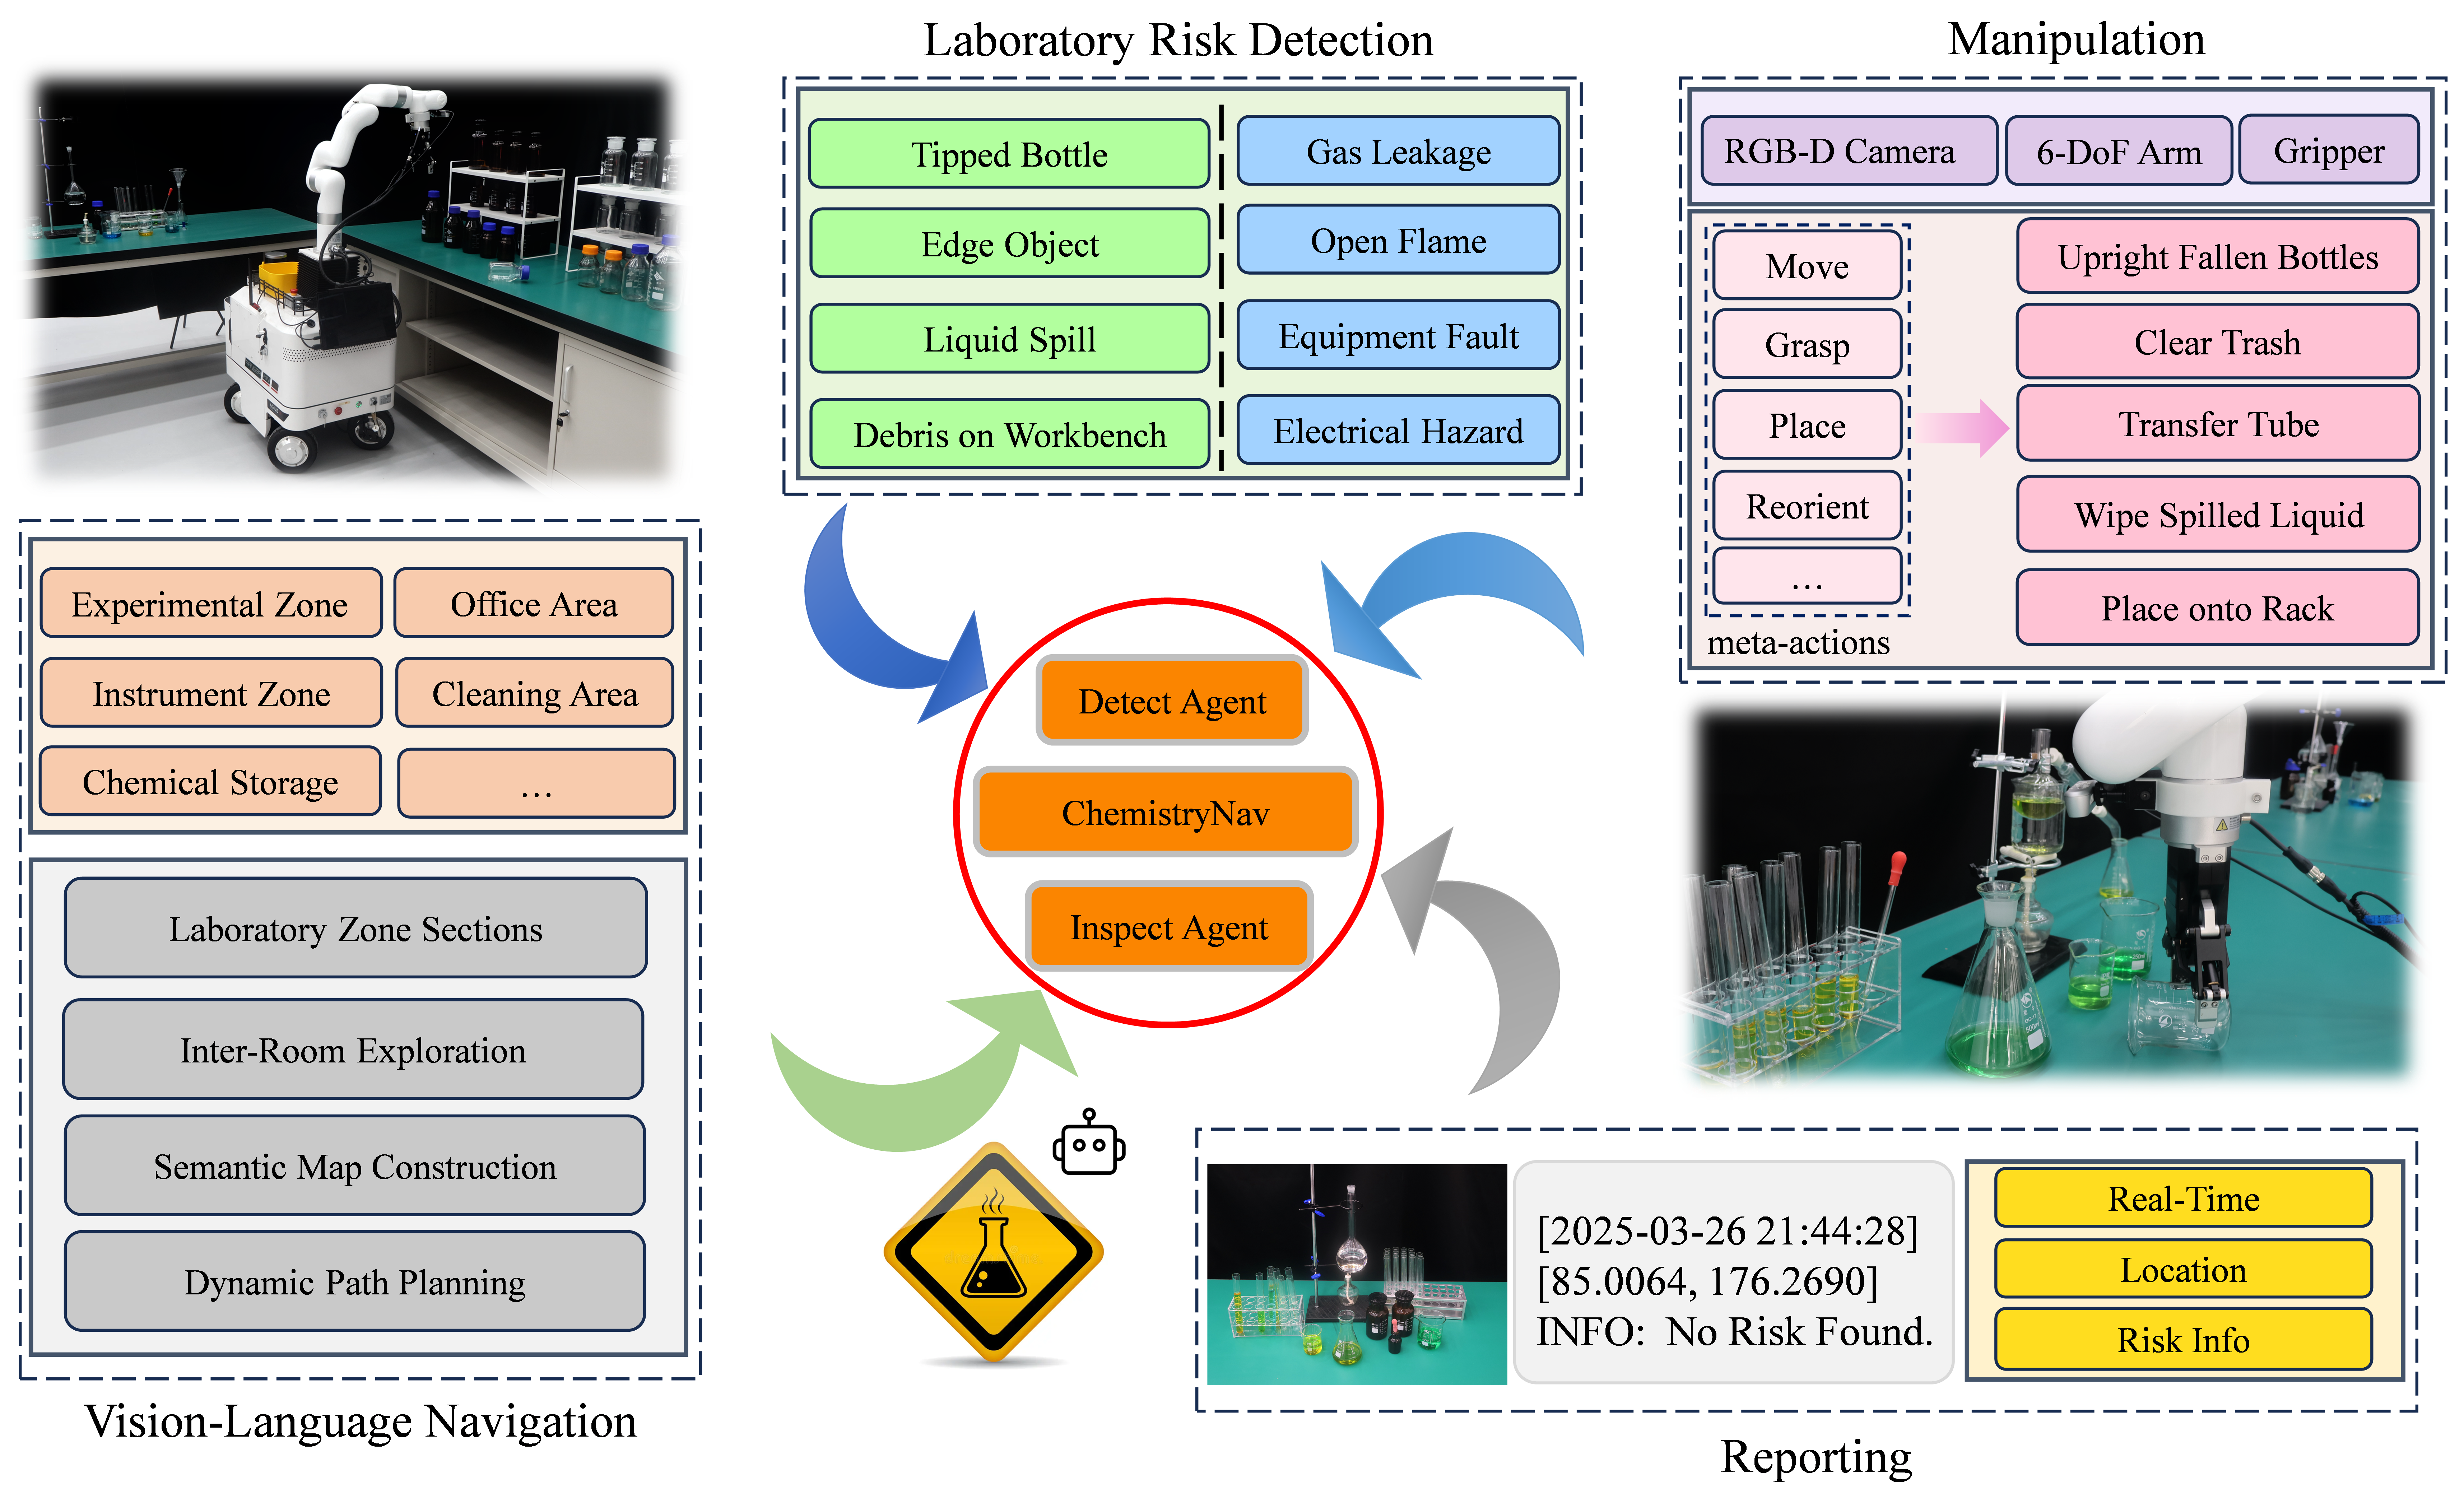
\includegraphics[width=1\textwidth]{figures/sys-overview.png}
  \caption{化学实验室安全巡检系统架构}
  \label{fig:sys-overview}
\end{figure}

如图\ref{fig:Hardware}所示,整体系统采用轮式移动底盘搭载 6 自由度机械臂的移动操作本体
,配备激光雷达、双目 RGB-D 相机等多模态传感器以及板载计算单元,
通过 ROS 统一调度感知、规划与控制模块。
在硬件层面,差速/全向复合运动能力的底盘保证了在狭窄走廊与仪器缝隙中的可达性,
高视场角 3D LiDAR 提供高精度二维/三维栅格建图与定位能力,
前向与臂载 RGB-D 相机分别承担室内布局感知与近距离操作观测任务,
6-DoF 机械臂与自适应夹爪则支撑包括扶正瓶体、移除边缘物体、擦拭液体、清理台面垃圾、试剂分类与试管转移在内的多种风险干预动作。
通过这种“底盘+臂+多模态感知”的本体设计,为后续在同一框架下统一处理移动与操作决策、实现语言驱动的具身移动操作提供了物理基础。

\begin{figure}[h]
  \centering
  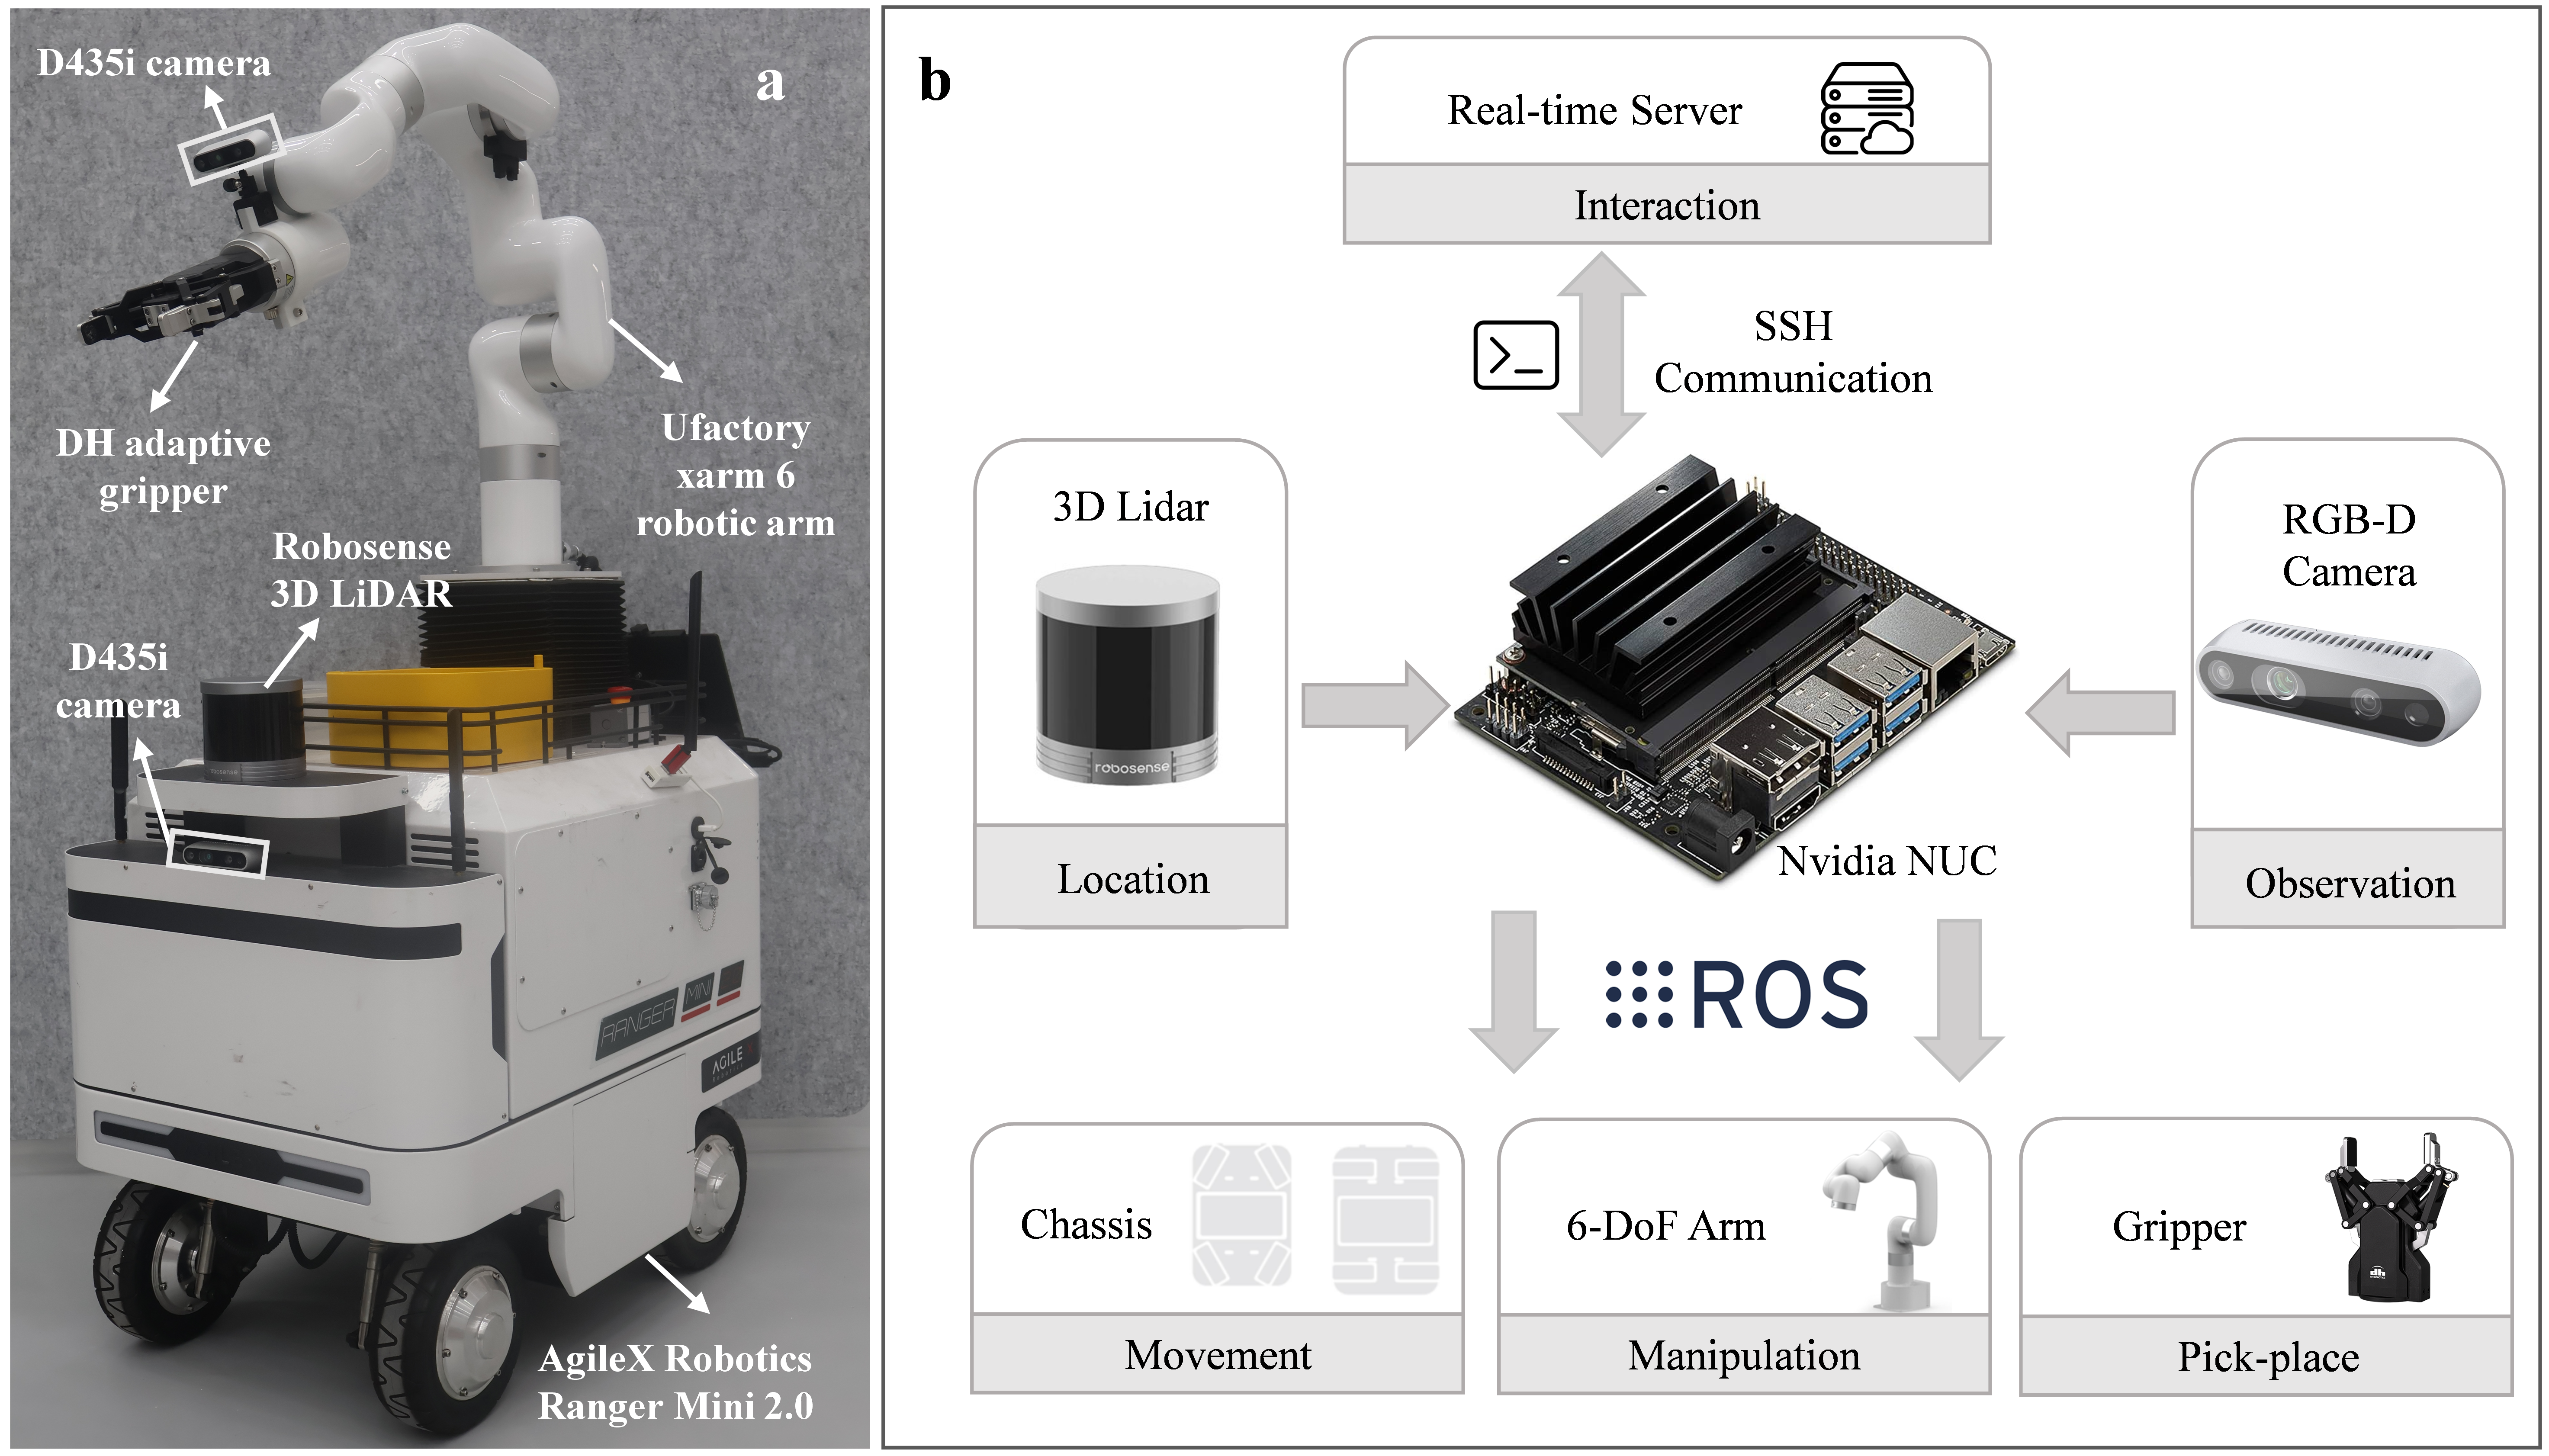
\includegraphics[width=0.8\textwidth]{figures/Hardware.png}
  \caption{系统硬件架构}
  \label{fig:Hardware}
\end{figure}

在导航与场景理解方面,提出了基于 Vision-and-Language Navigation(VLN)的 ChemistryNav 导航框架,如图\ref{fig:ChemistryNav}所示:
上层以大规模预训练 VLM 为核心,通过“指令–图像–历史轨迹”联合编码的方式,在语言指令约束下输出离散导航动作序列;
下层则结合 LiDAR-SLAM 提供的精准位姿与占据栅格地图,实现全楼层范围内的覆盖式探索与高精度建图。
与传统仅依赖几何信息的导航不同,ChemistryNav 在探索过程中持续构建细粒度语义地图,
将房间、走廊、实验区、储药区、清洗区等功能区域标注到同一地图坐标系中,实现“从语言到可达语义位点”的对齐。

\begin{figure}[h]
  \centering
  \includegraphics[width=1.0\textwidth]{figures/ChemistryNav.png}
  \caption{ChemistryNav 视觉-语言导航结构图与高精度语义地图构建示意图}
  \label{fig:ChemistryNav}
\end{figure}


在风险识别与语义推理方面,系统构建了视觉检测与实验室场景专用 VLM 推理的两级风控模块。
如图\ref{fig:RiskDetection}所示,考虑到实验室环境中透明容器、遮挡与杂乱布局带来的检测难度,视觉检测模块采用旋转框检测网络,
并通过实拍数据、公共实验室图像数据与基于 CAD 渲染的透明器皿合成数据构建混合训练集,
使模型在透明瓶、烧杯、三角瓶等目标上的检测精度显著提升。
检测结果被整理为结构化 JSON,其中包含每个目标的类别、中心位置、朝向等信息。
随后,这些结构化视觉信息与原始图像、预定义风险知识共同输入到基于 InternVL 微调的 Detect Agent,
由其完成“从物体组合到风险语义”的推理。通过“检测+VLM 推理”的方式,可以在不依赖人工规则库的前提下实现细粒度、多类型的风险识别,
为后续具身干预提供可靠语义输入。

\begin{figure}[h]
  \centering
  \includegraphics[width=0.9\textwidth]{figures/detection.png}
  \caption{风险识别与语义推理示意图}
  \label{fig:RiskDetection}
\end{figure}

面向“从风险语义到具身干预”的移动操作闭环,系统设计了 Inspect Agent 作为高层决策核心,将检测到的风险信息映射为一组可执行的双臂操作元动作序列。
具体来说,Inspect Agent 接收 Detect Agent 输出的风险类型、位置和上下文信息,通过提示工程与风险字典相结合的方式,
将风险匹配到“可操作风险模板”或“仅报告风险”两类;对于可操作风险,系统为每类风险预定义一簇可参数化的 meta-action 模板,
每个 meta-action 通过一套 API 映射到底层 Whole-Body 控制器的任务目标,
包括末端目标位姿求解、接近路径与中间 waypoint 生成、高度约束与避障约束设置、夹爪开合控制等。
执行过程中,搭载在机械臂上的 RGB-D 相机用于实时修正目标深度与姿态估计,控制器则根据点云和栅格地图动态调整臂姿与底盘姿态,
在保证避障和安全距离的前提下完成操作。

\begin{figure}[h]
  \centering
  \includegraphics[width=0.9\textwidth]{figures/manipulation.png}
  \caption{Inspect Agent 操作规划与执行示意图}
  \label{fig:InspectAgent}
\end{figure}

从本课题的角度看,这一面向实验室场景的移动操作系统设计,
实际上构成了“基于 VLM/VLA 的语义–几何中间表征、导航–操作协同决策以及数据–模型–场景闭环评估”的一个完整实例:
一方面,它提供了高精度导航、语义建图、风险识别与标准化操作原语等可复用模块,
为后续扩展到更一般的家庭与仓储场景、引入统一的 VLA 中间表征与跨场景训练策略奠定了工程基础;
另一方面,在真实复杂实验室环境中的长期运行,
也为本课题后续研究“如何在通用场景中构建稳定可靠的 VLA 驱动移动操作策略”提供了经验反馈。


\section{双臂协同精细操作决策方法}

在上述实验室移动操作系统中,虽然已经能够完成从语义驱动导航到基础风险干预的一整套流程,
但对于需要高精度对位、细小特征识别或受遮挡严重的操作场景,仅依赖单个视角和单臂操作仍然存在明显瓶颈:
一方面,台面杂物、仪器遮挡以及透明容器等因素导致关键接触区域难以稳定出现在视野中,
视觉分辨率与视角质量不足直接削弱了末端位姿估计与接触点选取的精度;
另一方面,许多场景下的操作任务天然具有双手协同特征,单臂策略往往需要冗长的动作序列才能近似完成,人机演示中也易出现抖动和次优轨迹,
给策略学习带来噪声。

为缓解这些问题,本课题在双臂平台上引入“主动视觉驱动的双臂协同精细操作”框架:
如图\ref{fig:avr-overview}所示,系统采用“直观数据采集-模型设计与训练-系统评估”的闭环流程,设计了多种双臂协同的精细操作任务,
并在各种场景下评估其鲁棒性与泛化性。

\begin{figure}[h]
  \centering
  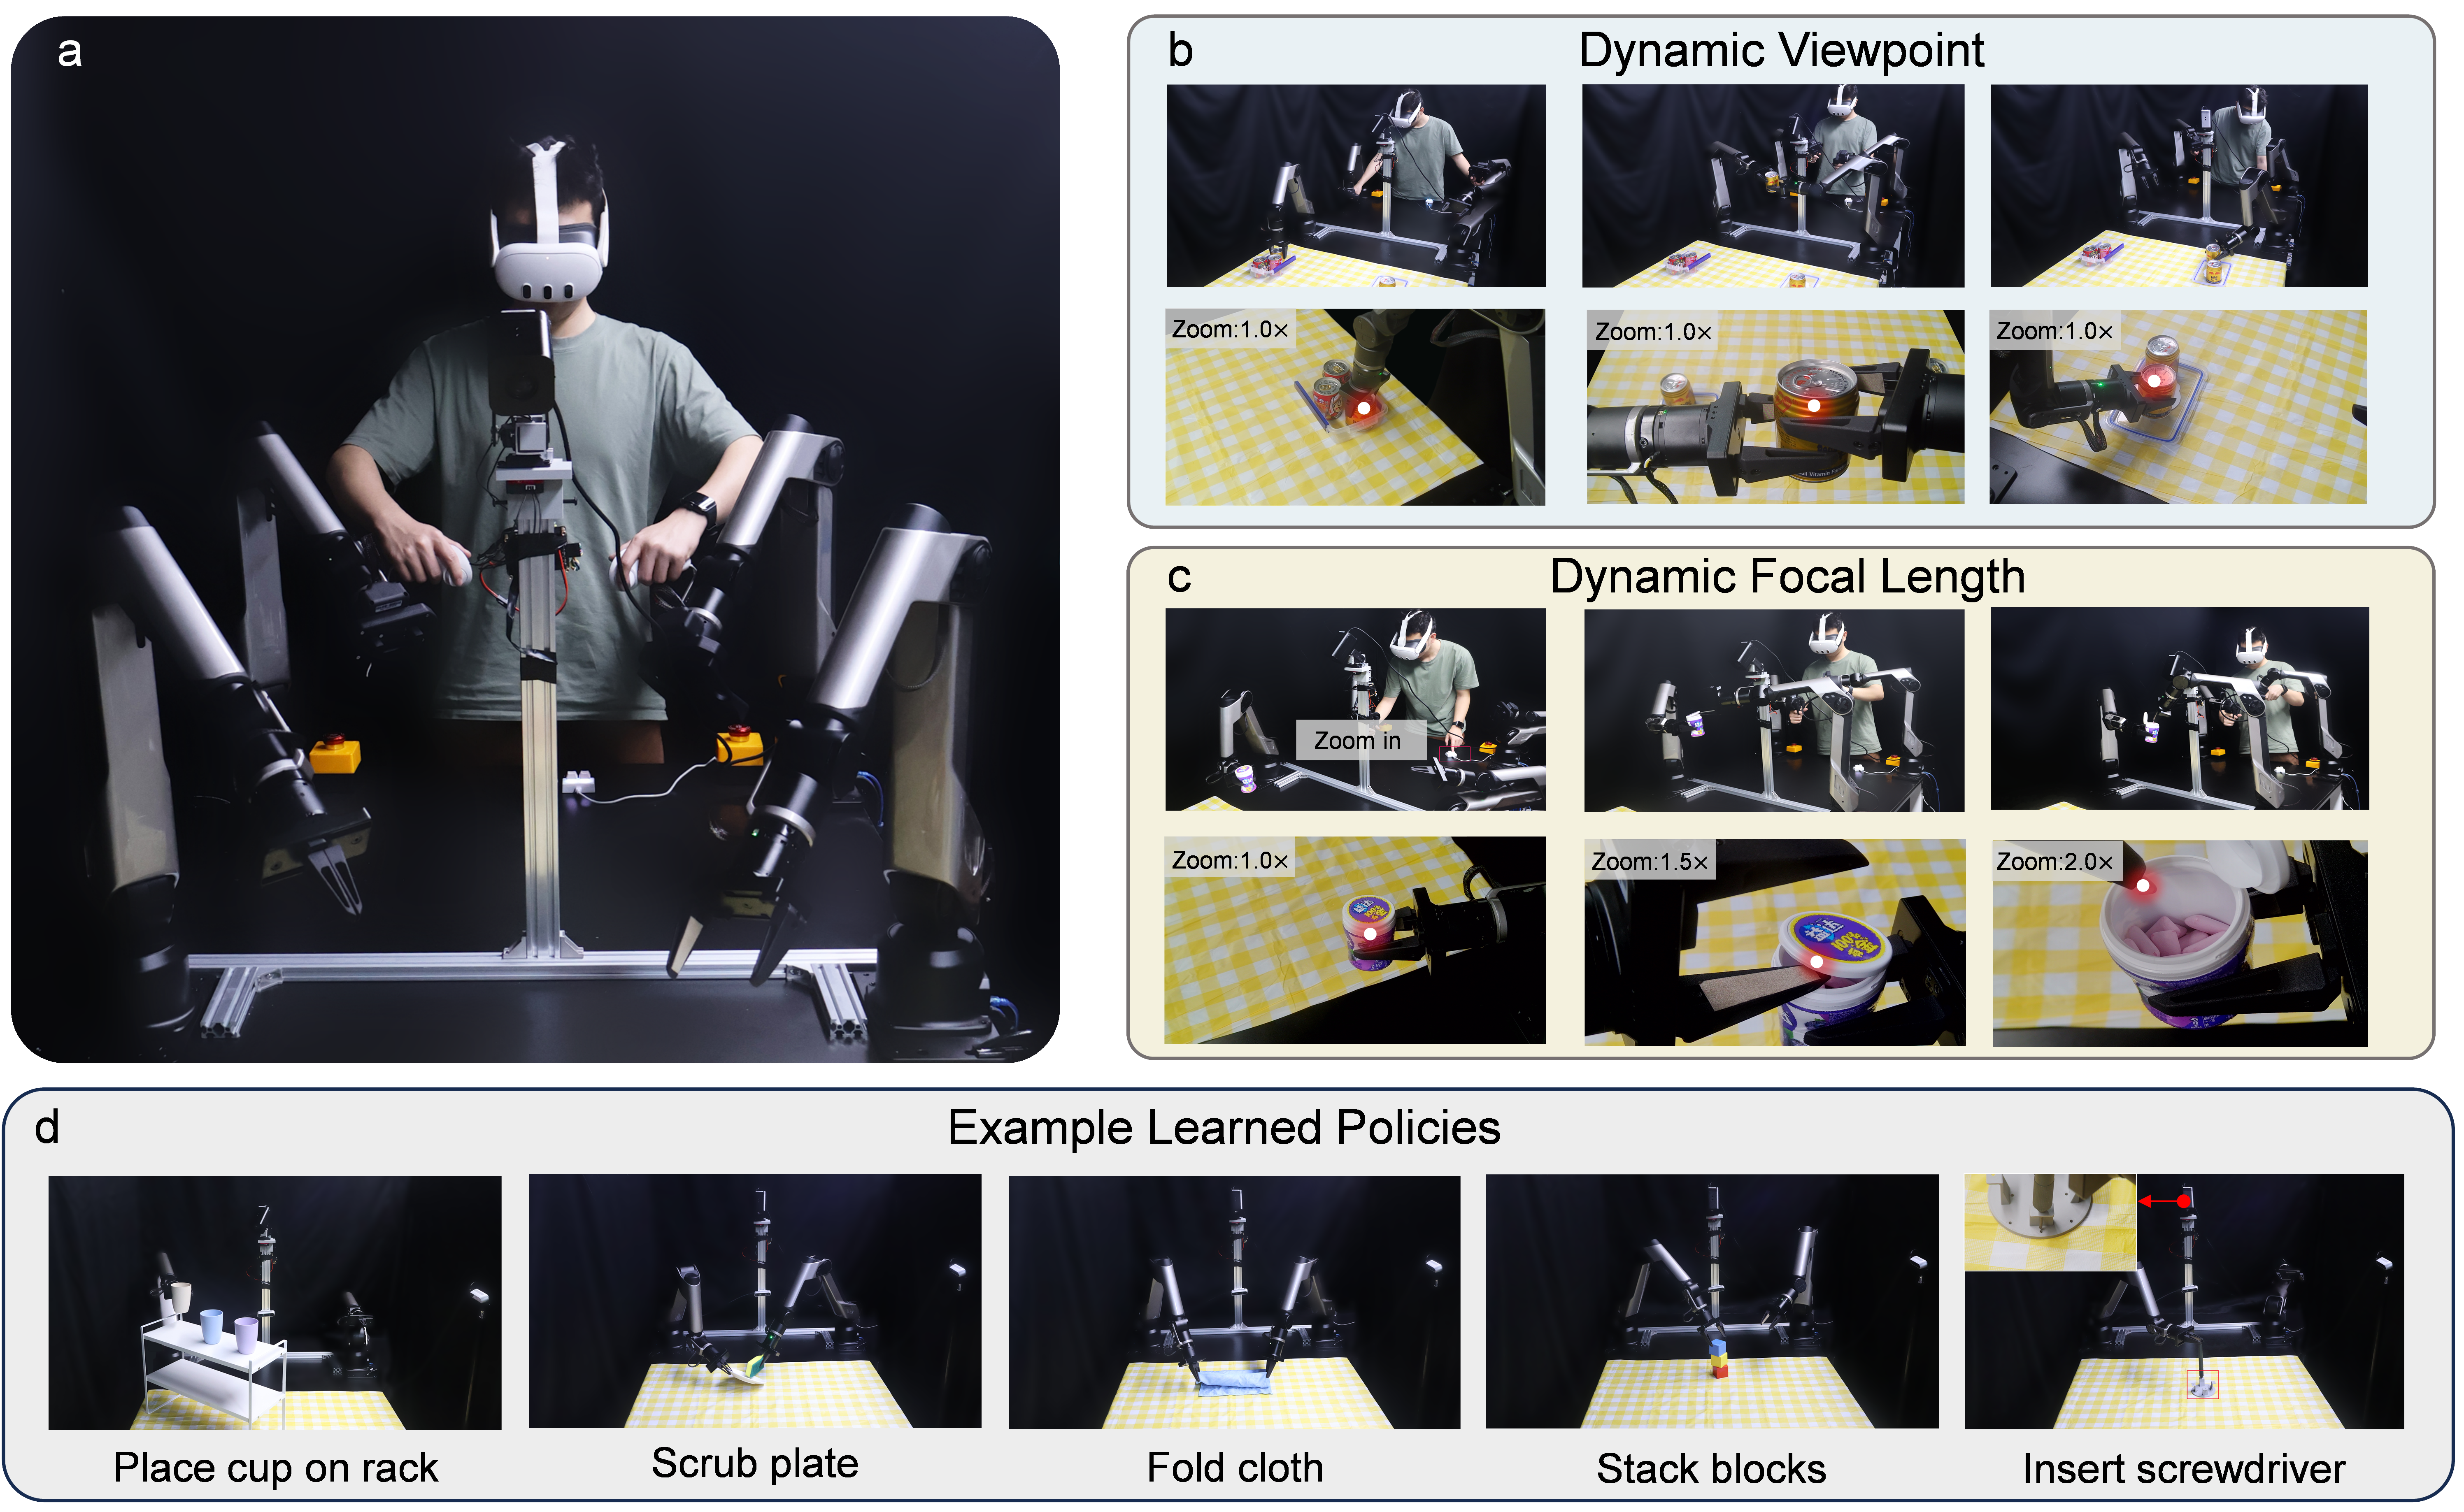
\includegraphics[width=1.0\textwidth]{figures/avr-overview.png}
  \caption{主动视觉驱动的双臂协同精细操作框架}
  \label{fig:avr-overview}
\end{figure}

在数据采集阶段,设计了基于第一视角的主从臂数据采集系统,如图\ref{fig:avr-architecture}所示:
通过将头戴式显示器的姿态映射到 2-DoF “主动视觉”云台,示教器设计焦距控制按钮来联动电动变焦工业相机,
使操作者能够像人类日常操作那样始终围绕任务关键部位进行“看近、看清、看准”的观察;
系统基于时间戳同步,记录包括多个相机实时RGB-D观测、双臂末端位姿、夹爪状态、云台角度与变焦倍率等多模态轨迹,
将这些细节观测与动作一起作为策略学习的输入,从源头上提升数据质量和对精细交互细节的覆盖度。

\begin{figure}[h]
  \centering
    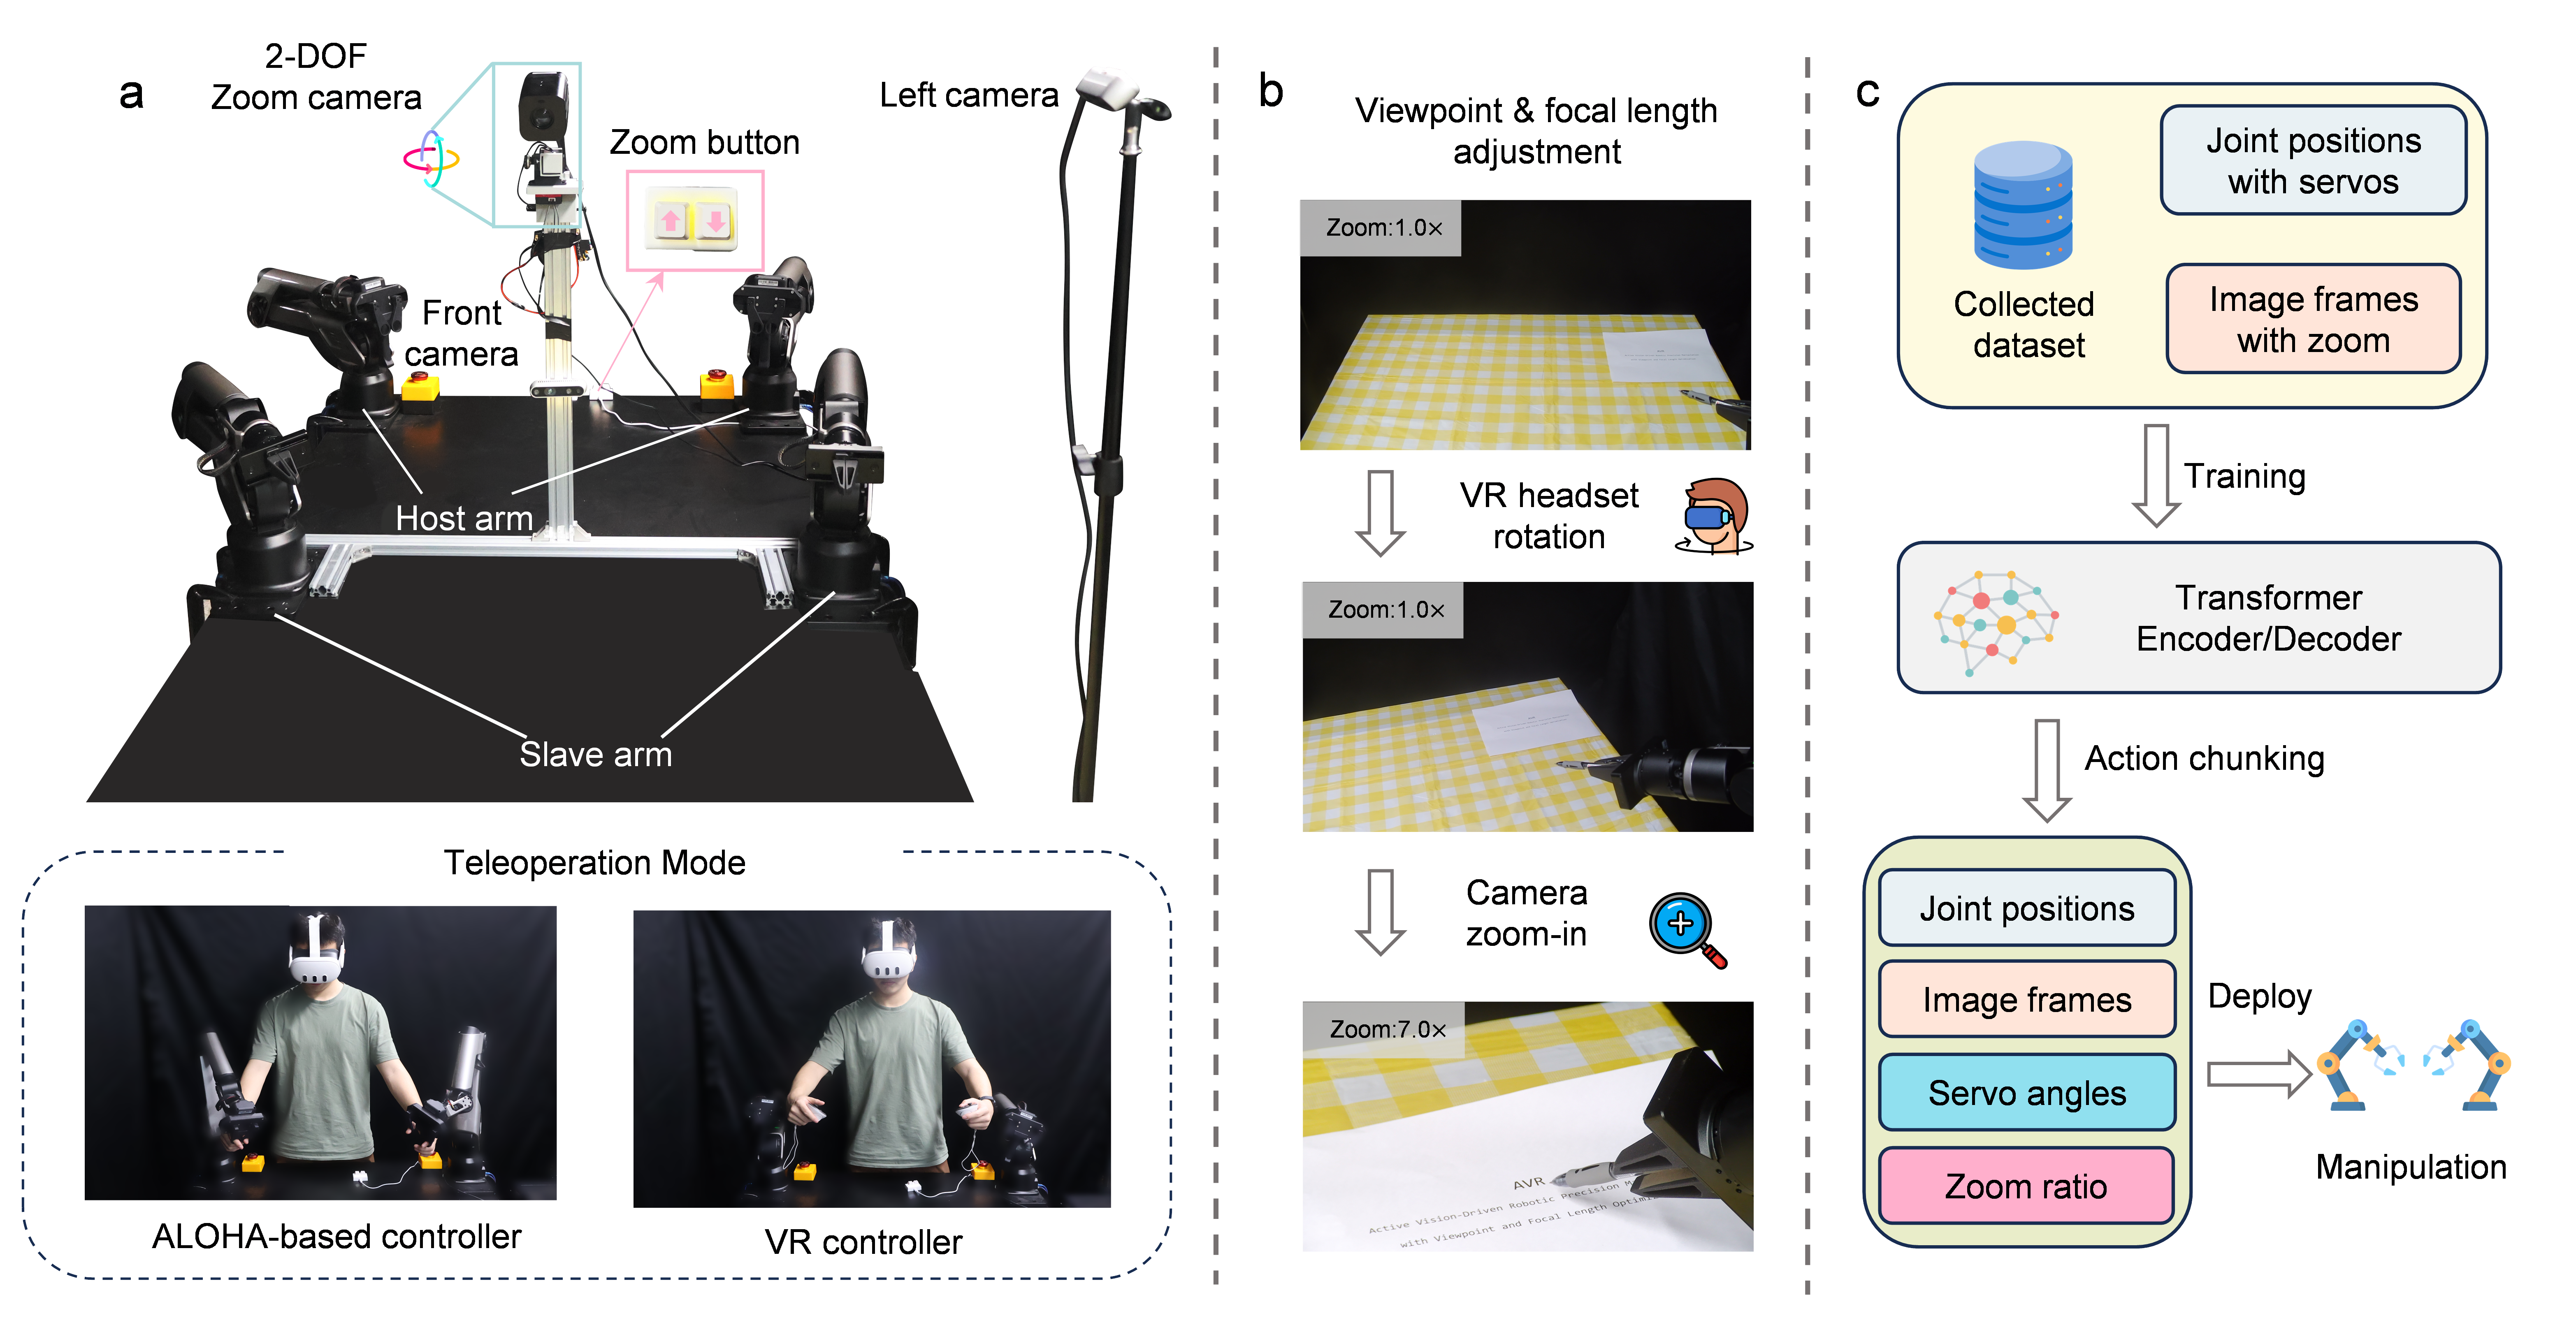
\includegraphics[width=1.0\textwidth]{figures/avr-architecture.png}
  \caption{数据采集系统与系统架构示意图}
  \label{fig:avr-architecture}
\end{figure}

在模型设计与训练阶段,系统设计了多种双臂协同的精细操作任务,并采用了基于模仿学习方法
(如ACT\citep{Zhao2023Learning}, DP3\citep{Ze20243DPolicy}等)
和VLA方法(如$\pi_0$\citep{Black2024pi_0}, OpenVLA\citep{Kim2024OpenVLA}等)进行微调的策略学习方法,
以实现从数据中学习双臂协同的精细操作策略。
在策略学习与在线决策阶段,双臂协同的精细操作被统一建模为“感知–主动观测–双臂协调”一体化过程:
基于扩散策略等数据驱动方法,策略网络同时接收外部多视角图像、主动视觉相机输出和本体状态,
在高维观测空间中首先确定当前任务阶段与关键接触区域,随后联合输出两臂末端轨迹、夹爪开合、云台转动与变焦控制等连续动作,
使“视角选择”和“手部动作”在统一策略中协同演化。

\begin{figure}[h]
  \centering
  \includegraphics[width=0.9\textwidth]{figures/avr-evaluation.png}
  \caption{真实环境中的系统部分评估结果}
  \label{fig:avr-evaluation}
\end{figure}

在系统评估阶段,分别设计了基于RoboTwin2.0的仿真环境与真实实验室环境的评估方法,
通过在仿真环境中设计“主动视觉插件”,设计并模拟各种场景下的双臂协同精细操作任务,并与未添加主动视觉方法的baseline进行比较,
从而评估主动视觉方法在双臂协同精细操作任务中的有效性。
同时在真实环境中,通过在线部署预训练的策略模型,在各类典型任务上进行系统评估。
如图\ref{fig:avr-evaluation}所示,实验结果表明,相比于固定视角、单臂或仅视角可动的基线方法,引入双臂协同与主动视觉之后,
在相同或更少演示数据条件下,策略在高精度操作任务中的成功率和鲁棒性均显著提升,
对遮挡、杂乱和光照扰动的敏感度明显降低,
也为后续将该类精细操作能力嵌入移动操作系统的完整闭环奠定了方法基础。


\section{通用移动操作任务Benchmark构建}

要进一步推动具身移动操作在更广泛通用场景中的发展,就必须摆脱“单场景、单任务、单平台”的评测局限,构建具有代表性、可复现、可扩展的通用移动操作 Benchmark。
我们拟从“任务–场景–平台–指标”四个维度出发,构建基于轮式双臂平台的,面向通用室内环境的移动操作 Benchmark:
\begin{itemize}
  \item 在任务层面,以实验室安全排查、家居物体整理、仓储取放等典型应用为蓝本,将“语义导航 + 视角重配置 + 单/双臂操作”的长时序技能链条抽象为标准化任务模板;
  \item 在场景层面,围绕实验室、家庭、仓储等多类环境,设计具有不同空间结构、遮挡模式与风险要素分布的模拟与真实场景组,并保证任务在不同场景之间具备可对齐的难度分级与语义结构;
  \item 在平台层面,面向轮式双臂移动操作本体与仿真代理统一接口与状态–动作空间,使同一策略可以在“仿真–真机”“单臂–双臂”“室内–半结构化环境”之间迁移与对比;
  \item 在指标层面,则在传统的任务成功率、路径效率、操作精度基础上,引入风险识别与处置能力、主动视觉收益(如视角重配置前后观测不确定性下降)、跨场景迁移性能等综合指标,形成能够真实反映 VLA 驱动移动操作系统在通用场景下鲁棒性与实用性的评价体系。
\end{itemize}

现有的工作如BEHAVIOR-1K\citep{Li2023Behavior1K}等,对多种室内外操作场景进行了丰富的建模并开源:
如图\ref{fig:scene}所示,其包含 50 个场景(如房屋、花园、餐厅、办公室等),有超过 9,000 个对象进行了丰富的物理和语义属性标注,
并基于Omnibigson对刚体、可变形物体和液体的现实物理模拟和渲染。
在此基础上,我们拟基于此数据集,构建面向通用室内环境的移动操作 Benchmark,并在此基础上进行策略学习与评估。

\begin{figure}[h]
  \centering
  \includegraphics[width=1.0\textwidth]{figures/scene.png}
  \caption{BEHAVIOR-1K部分场景示意图}
  \label{fig:scene}
\end{figure}

基于轮式双臂平台的全身控制,以星海图R1本体为例,我们搭建了基于VR遥操作的数据采集装置,包含轮式底盘的移动和双臂协同的各类操作。
在具有多个关节组件的移动操作,相较于传统固定位置双臂控制,对移动模态的编码和理解,
若仅仅作为新的模态传入并交由现有SoTA VLA模型过拟合训练,会存在如数据理解弱、末端执行器偏差严重、操作不鲁棒等问题。
基于此,我们在基于学习的全身控制基础上,通过自回归全身动作解码(如图\ref{fig:wb-vima}所示),将上半身动作预测条件化于预测的下半身动作,
并独立设计去噪扩散网络,使得策略能够更好地建模协调的全身动作,减少误差传播。

\begin{figure}[h]
  \centering
  \includegraphics[width=1.0\textwidth]{figures/wb-vima.png}
  \caption{全身动作解码结构图}
  \label{fig:wb-vima}
\end{figure}

通过外部VR设备对仿真或真机的数据采集,并结合本体状态与动作,在Benchmark中进行策略学习与评估。
通过这样的 Benchmark 构建,一方面可以将本课题在实验室移动操作与双臂精细操作中的经验抽象为可共享的任务与场景资源,
降低后续研究的进入门槛;
另一方面也为不同算法和系统提供统一、公正的比较平台,
从而推动面向通用场景的具身移动操作方法向更加系统化、工程化和可落地的方向演进。


\section{技术路线总结}


综上所述,本章围绕“面向通用场景的基于视觉–语言–动作模型的具身移动操作方法”这一总体目标,
从系统实例、方法机制与评测体系三个层面给出了完整的研究方法与技术路线。
首先,基于化学实验室安全巡检与风险干预系统,构建了集高精度导航、语义建图、风险识别与标准化操作原语于一体的移动操作系统,
展示了如何在真实高风险场景下实现“从语言与视觉语义到具身移动操作”的闭环流程,为后续工作提供了可复用的硬件平台与软件架构。
其次,在双臂协同精细操作方向,引入“主动视觉驱动的双臂协同精细操作”框架,
通过第一视角与变视角/变焦距观测机制显著提升了精细操作数据的质量,
并利用模仿学习与 VLA 策略将“视角选择”和“双臂动作”统一建模为一体化决策过程,
从而补足了实验室场景中对高精度对位与复杂双手协作的关键能力。
再次,在通用移动操作任务 Benchmark 构建方面,面向实验室、家庭与仓储等多类室内环境,
从任务、场景、平台与指标四个维度设计了统一的评测框架,
并在轮式双臂本体上探索了自回归全身动作解码与仿真–真机联合数据采集训练策略,
为系统性比较不同 VLA 驱动移动操作方法及其跨场景泛化能力提供了实验基础。

总体来看,本章所提出的技术路线在“感知–决策–执行”的闭环之上,叠加了“数据–模型–场景”的迭代机制:
一方面,通过实验室移动操作系统与主动视觉双臂平台,将语义–几何中间表征、导航–操作协同决策与全身控制落地到真实机器人系统中;
另一方面,通过通用移动操作 Benchmark 的构建与仿真–真机对照实验,使得后续章节中的 VLA 表征设计、
协同决策方法与跨场景训练策略能够在统一基准下得到量化验证。
围绕本章所确立的研究方法与技术路线,后续工作将重点展开 VLA 中间表征的具体形式、高精度导航与精细操作一体化策略的设计与实现,
以及在通用室内任务集上的实验评估与算法对比,从而逐步实现面向通用场景的具身移动操作能力。
